% Provenance (never printed): see sources/outline_sources.md (Year 1: gravity and its
% measurement, normal gravity; isostasy, Airy and Pratt; free-air and Bouguer anomalies;
% the geoid). Curves from figdata/bachelor-1/hypsometry.py and gravity_profiles.py;
% exercise and problem values in the Book 3 scratch calculator calc/ch11.py.
\chapter{التوازن الأيزوستاتي وشذوذات الجاذبية}\label{ch:b1:isostasy-gravity}

في أربعينيات القرن التاسع عشر واجه المساحون الذين كانوا يقيسون قوسًا من خط الزوال في شمال الهند تناقضًا لم يستطيعوا عزوه إلى أدواتهم. فبين محطتين تبعد إحداهما عن الأخرى نحو 370 ميلًا، هما كاليانا قرب سفح الهملايا وكاليانبور بعيدًا نحو الجنوب، كان الفرق في \omterm{def:b1:spherical-astronomy:geographic}{العرض الجغرافي} الذي وجدوه بالتثليث أكبر من الفرق الذي وجدوه من النجوم بمقدار \num{5.236} ثانية قوسية. وكان المتّهم الواضح هو الجبال: فجاذبها يسحب الشاقول نحو الشمال، والفلكيون يضبطون أدواتهم على الشاقول. وفي 1855 حسب جون هنري برات جذب الهملايا والهضاب التي وراءها، فوجد أن التناقض كان يجب أن يبلغ \num{15.885} ثانية قوسية، أي أكثر من ثلاثة أضعاف ما لوحظ. إذن جذبت الجبال أقلّ بكثير مما كانت كتلتها المرئية تقتضيه. وفي العام نفسه أجاب جورج إيري بأن \omterm{def:b1:layered-earth:layers}{القشرة} تطفو على طبقة أكثف، كما تطفو طوافة من الجذوع على الماء، فيكون للمرتفعات جذر عميق من صخر خفيف. أما برات فاقترح لاحقًا جوابًا آخر: صخرًا أُخفّ بالتمدّد تحت الجبال. وكلا الجوابين ما زال يُدرَّس، فالجبال تستند إلى صخر خفيف يعوّض كتلتها. يحوّل هذا الفصل الفكرة إلى أرقام، ويبيّن كيف تكشف الجاذبية، التي تُقاس بدقة جزء من المليون من قيمتها، الكتلَ المخفية تحت التضاريس.
% ledger: pratt:himalaya, airy:1855, pratt:1871

\begin{recall}
ينص قانون نيوتن للجذب على أن مجال الجاذبية $g = GM/r^2$ خارج كتلة كروية $M$؛ ويشتق هذا المجال من جهد للجاذبية، وسطح تساوي الجهد عمودي في كل نقطة على المجال (الفيزياء). وفي مائع ساكن يزداد الضغط مع العمق وفق $\mathrm dp/\mathrm dz = \rho g$، والجسم العائم يزيح وزنه من المائع (الفيزياء؛ السنة الجامعية الأولى). وتحت \omterm{def:b1:layered-earth:lithosphere}{الغلاف الصخري} يتدفّق \omterm{def:b1:layered-earth:lithosphere}{الغلاف اللدن} ببطء على مدى أزمنة طويلة؛ \omterm{def:b1:layered-earth:layers}{والقشرة} أخفّ من \omterm{def:b1:layered-earth:layers}{الوشاح} الذي تحتها (\cref{ch:b1:layered-earth}؛ الكتاب 2، الصف 11).
\end{recall}

\section{الجاذبية وقياسها}

تبلغ جاذبية الأرض عند سطحها قرابة \qty{9.8}{m.s^{-2}}، أما التغيّرات التي تهمّ الجيولوجيين فأصغر منها بنحو مليون مرة. وتُعدّ بوحدة من منظومة السنتيمتر والغرام القديمة هي الغال: $\qty{1}{Gal} = \qty{1}{cm.s^{-2}} = \qty{0.01}{m.s^{-2}}$، بحيث
\[
  \qty{1}{\milli\gal} = \qty{e-5}{m.s^{-2}} \approx \num{e-6}\,g .
\]
% ledger: nist:gal
يميّز الجهاز الحقلي بضعة أجزاء من الألف من الميليغال؛ وتتراوح الشذوذات التي تدرسها هذه الفصل بين جزء من الميليغال فوق جسم خامٍ مدفون، وبضع مئات من الميليغالات فوق سلسلة جبلية.

حتى على أرض لا تختلف ملامحها لن تكون الجاذبية واحدة في كل مكان. فالأرض تدور، فما يحسّ به الشاقول أو مقياس الجاذبية هو مجموع الجذب الثقالي والأثر الطارد المركزي للدوران؛ والأرض مفلطحة، فالقطبان أقرب إلى مركزها من خط الاستواء. ويُضعف الأثران الجاذبية عند خط الاستواء عنها عند القطبين. ويقارن الجيولوجي كل قياس بمرجع أملس يشملها.

\begin{definition}[الجاذبية المرجعية]\label{def:b1:isostasy-gravity:normal-gravity}
\emph{الجاذبية المرجعية}\index{الجاذبية المرجعية} $\gamma$ هي جاذبية أرض نموذجية: قطع ناقص دوراني له كتلة الأرض ودورانها، يُختار بحيث يكون سطحه سطح تساوي جهد لجاذبيته هو (الجذب الثقالي مع الأثر الطارد المركزي). وعلى ذلك السطح تتعلّق الجاذبية المرجعية \omterm{def:b1:spherical-astronomy:geographic}{بالعرض الجغرافي} وحده.
\end{definition}

لن يُدرس القطع الناقص نفسه، ولا تفلطحه، ولا طريقة ملاءمة معاييره للأرض الحقيقية، إلا في الكتاب 5. وهنا نحتاج إلى جاذبيته وحدها.

\begin{proposition}[صيغة الجاذبية المرجعية]\label{prop:b1:isostasy-gravity:normal-formula}
على القطع الناقص المرجعي المعتمد عام 1980، تكون \omterm{def:b1:isostasy-gravity:normal-gravity}{الجاذبية المرجعية} عند \omterm{def:b1:spherical-astronomy:geographic}{العرض الجغرافي} $\varphi$، في صورتها المتسلسلة المعتادة،
\[
  \gamma(\varphi) = \qty{9.780327}{m.s^{-2}}\,\bigl(1 + 0.0053024\sin^2\varphi
  - 0.0000058\sin^2 2\varphi\bigr).
\]
\end{proposition}
\admitted
% ledger: moritz:grs80

فهي تعطي \qty{9.780327}{m.s^{-2}} عند خط الاستواء، و\qty{9.806200}{m.s^{-2}} عند \ang{45}، و\qty{9.832186}{m.s^{-2}} عند القطبين: الفرق من خط الاستواء إلى القطب \qty{5186}{\milli\gal}. ويعود معظم هذا الفرق إلى الدوران وحده. ومع اليوم النجمي البالغ \qty{23.9345}{h} تكون السرعة الزاوية $\omega = 2\pi/\qty{86164}{s} = \qty{7.292e-5}{rad.s^{-1}}$، والتسارع الطارد المركزي عند خط الاستواء، $\omega^2 a$ مع $a = \qty{6378.137}{km}$، هو \qty{0.0339}{m.s^{-2}}، أي \qty{3392}{\milli\gal}؛ ويوفّر التفلطح الباقي (\cref{exo:b1:isostasy-gravity:2}).
% ledger: earth:Trot, earth:Req, earth:geq, earth:gpole

تُقاس الجاذبية بطريقتين. فالمقياس \emph{المطلق} يُسقط كتلة اختبار في حجرة مفرغة، ويتتبّع سقوطها الحر بمقياس تداخل ليزري، ويُوقَّت بساعة ذرّية، فيخرج التسارع مباشرة من المسافة والزمن. أما المقياس \emph{النسبي} فهو كتلة معلّقة بنابض يتغيّر امتداده مع الجاذبية؛ وهو خفيف وسريع، لكنه لا يعطي إلا الفروق بين الأماكن، ويتزحزح مع الزمن، فيعود المسح إلى محطة أساس تُعرف جاذبيتها. وأدق المقاييس المطلقة تبلغ دقة نحو ميكروغال، أي جزءًا من مليار من $g$.
% ledger: ngs:absolute-gravity

\begin{inthefield}[مسح للجاذبية على اليابسة]
\begin{minipage}[t]{0.55\linewidth}\vspace{0pt}
مسح الجاذبية مشيٌ بطيء من محطة إلى أخرى. يضع الجيوفيزيائي عند كل محطة مقياس الجاذبية النسبي على حامله الثلاثي، ويسوّيه، وينتظر استقرار النابض ويأخذ عدّة قراءات؛ ويسجّل مستقبل تحديد المواقع بالأقمار الصناعية المجاور موقع المحطة وارتفاعها. وكل بضع ساعات يعود الفريق إلى محطة الأساس، ليُقاس انزياح النابض ويُزال. والارتفاع لا يقلّ أهمية عن الجاذبية: فكما يبيّن القسم التالي، تنخفض الجاذبية بمقدار \qty{0.3086}{\milli\gal} لكل متر ارتفاع، فيكفي ارتفاع خاطئ بمقدار \qty{1}{cm} ليُفسد القراءة بمقدار \qty{3}{\micro\gal}. % ledger: usgs73:reduction
\end{minipage}\hfill
\begin{minipage}[t]{0.42\linewidth}\vspace{0pt}
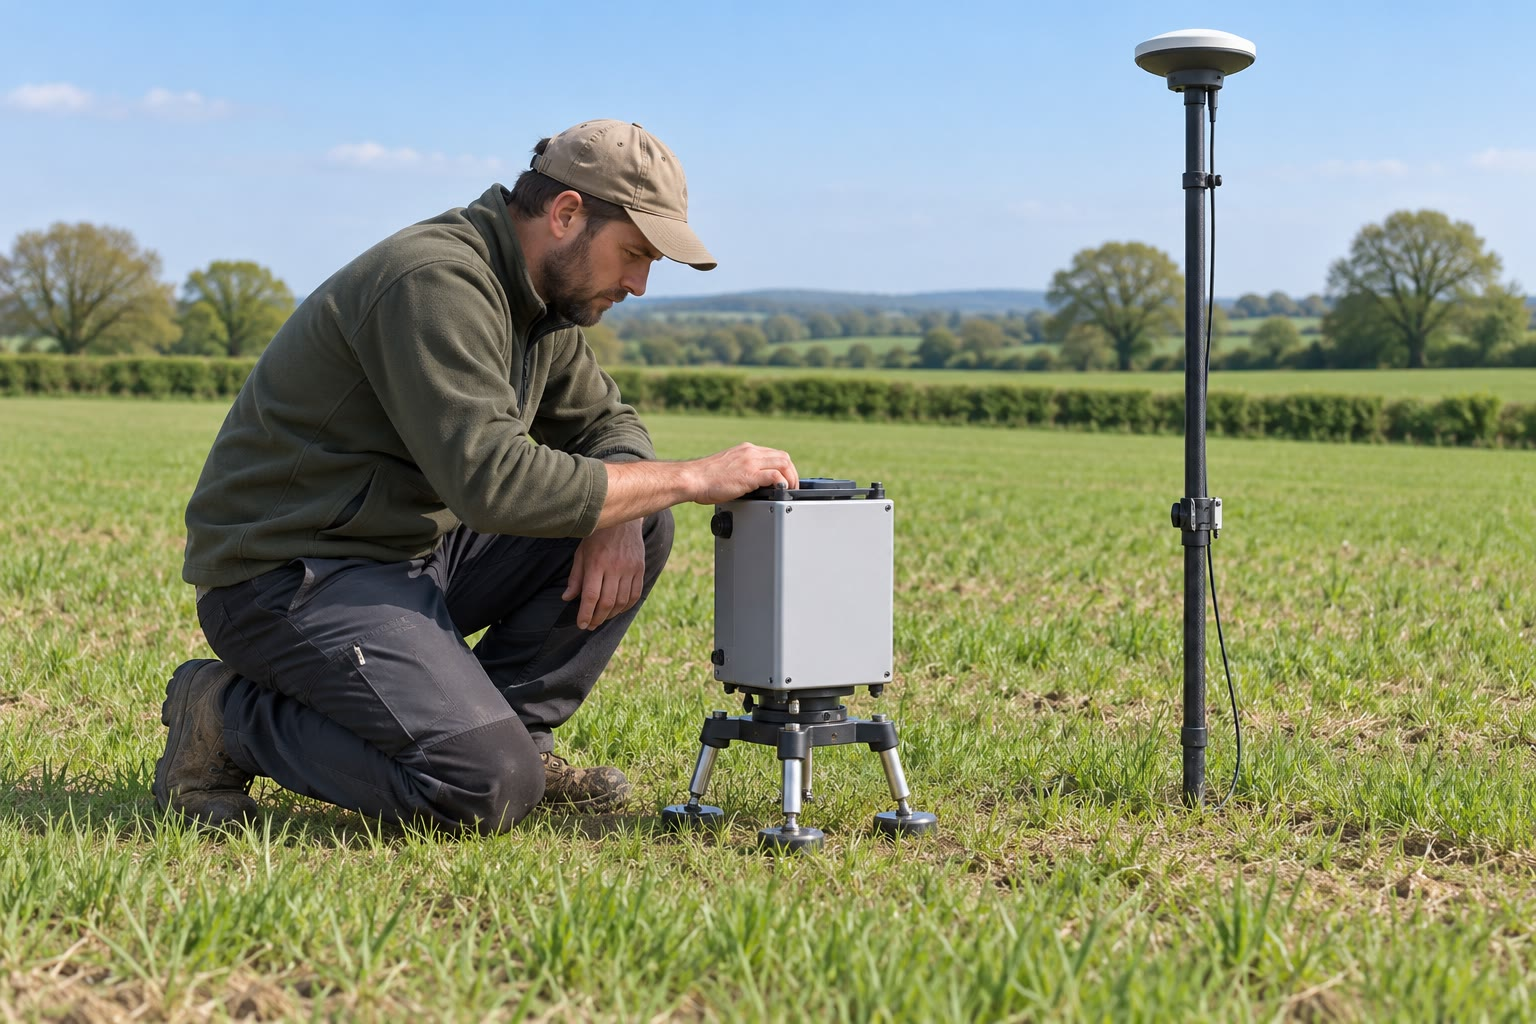
\includegraphics[width=\linewidth]{images/book3/ai/b1-gravity-survey.jpg}

{\scriptsize مقياس جاذبية حقلي على حامله الثلاثي، وإلى جانبه هوائي تحديد المواقع بالأقمار الصناعية (رسم توضيحي بالذكاء الاصطناعي).}
\end{minipage}
\end{inthefield}

\section{التوازن الأيزوستاتي}

التعويض الذي تصوّره إيري وبرات للهملايا مثال على حالة عامة للطبقات الخارجية للأرض.

\begin{definition}[التوازن الأيزوستاتي؛ عمق التعويض]\label{def:b1:isostasy-gravity:isostasy}
تكون المنطقة في \emph{التوازن الأيزوستاتي}\index{التوازن الأيزوستاتي}، أي في حالة توازن أيزوستاتي، حين يوجد عمق، هو \emph{عمق التعويض}\index{عمق التعويض}، يكون الضغط عنده واحدًا عند كل نقطة من السطح الأفقي، مهما كانت التضاريس فوقه. وتحت عمق التعويض تسلك الصخور سلوك مائع ساكن؛ وفوقه تطفو عليه أعمدة \omterm{def:b1:layered-earth:layers}{القشرة} \omterm{def:b1:layered-earth:layers}{والوشاح}.
\end{definition}

\begin{proposition}[كتلتان متساويتان فوق عمق التعويض]\label{prop:b1:isostasy-gravity:equal-mass}
إذا كانت الجاذبية $g$ واحدة على امتداد كل الأعمدة، تكون المنطقة في \omterm{def:b1:isostasy-gravity:isostasy}{التوازن الأيزوستاتي} \omterm{def:b1:isostasy-gravity:isostasy}{بعمق التعويض} $z_c$ إذا وفقط إذا احتوى كل عمود شاقولي مقطعه وحدة المساحة، من السطح حتى $z_c$، الكتلة نفسها.
\end{proposition}

\begin{proof}
في كل عمود تكون الصخور في توازن هيدروستاتيكي، بحيث $\mathrm dp/\mathrm dz = \rho(z)\,g$، مع عدّ العمق $z$ نحو الأسفل. ويكون الضغط عند السطح جويًا، واحدًا في كل مكان (وهو مهمل). وبالتكامل من السطح $z_s$ للعمود حتى $z_c$ نجد:
\[
  p(z_c) = p_0 + g\int_{z_s}^{z_c}\rho(z)\,\mathrm dz ,
\]
حيث يمثّل التكامل كتلة العمود لكل وحدة مساحة. والضغطان عند $z_c$ متساويان إذا وفقط إذا تساوت هاتان الكتلتان.
\end{proof}

توزيعان بسيطان للكتل يعطيان النموذجين الكلاسيكيين (الشكل أدناه).

\begin{proposition}[توازن إيري]\label{prop:b1:isostasy-gravity:airy}
لتكن \omterm{def:b1:layered-earth:layers}{القشرة} ذات كثافة منتظمة $\rho_c$ وسمك $H$ حيث يكون سطحها عند مستوى البحر، فوق \omterm{def:b1:layered-earth:layers}{وشاح} كثافته $\rho_m > \rho_c$. في \omterm{def:b1:isostasy-gravity:isostasy}{التوازن الأيزوستاتي}:
\begin{enumerate}
  \item حيث يقع السطح على ارتفاع $h$ فوق مستوى البحر، تملك \omterm{def:b1:layered-earth:layers}{القشرة} جذرًا عمقه $r = h\,\rho_c/(\rho_m - \rho_c)$ تحت \omterm{def:b1:layered-earth:layers}{القشرة} العادية، وسمكها $H + h + r$؛
  \item حيث يقع السطح على عمق $d$ تحت مستوى البحر، تحت ماء كثافته $\rho_w$، تملك \omterm{def:b1:layered-earth:layers}{القشرة} جذرًا معكوسًا: تُرفع قاعدتها بمقدار $r' = d\,(\rho_c - \rho_w)/(\rho_m - \rho_c)$، ويكون سمكها $H - d - r'$.
\end{enumerate}
هذا هو \emph{توازن إيري}\index{توازن إيري}: تعويض بتغيّر السمك عند كثافة ثابتة.
\end{proposition}

\begin{proof}
نأخذ \omterm{def:b1:isostasy-gravity:isostasy}{عمق التعويض} مباشرةً تحت أعمق جذر، ونقارن كل عمود بالعمود العادي. (1) للعمود المرتفع \omterm{def:b1:layered-earth:layers}{قشرة} بدل \omterm{def:b1:layered-earth:layers}{الوشاح} على العمق $r$، \omterm{def:b1:layered-earth:layers}{وقشرة} على الارتفاع $h$ حيث لا شيء في العمود العادي: تقتضي تساوي الكتلتين أن $\rho_c(h + r) = \rho_m r$، أي $r(\rho_m - \rho_c) = \rho_c h$. (2) للعمود المنخفض ماء بدل \omterm{def:b1:layered-earth:layers}{القشرة} على العمق $d$، \omterm{def:b1:layered-earth:layers}{ووشاح} بدل \omterm{def:b1:layered-earth:layers}{القشرة} على $r'$: يقتضي تساوي الكتلتين أن $\rho_w d + \rho_m r' = \rho_c(d + r')$، أي $r'(\rho_m - \rho_c) =
d(\rho_c - \rho_w)$.
\end{proof}

\begin{proposition}[توازن برات]\label{prop:b1:isostasy-gravity:pratt}
لتنتهِ كل الأعمدة عند \omterm{def:b1:isostasy-gravity:isostasy}{عمق التعويض} نفسه $D$ تحت مستوى البحر، بكثافة منتظمة في كل عمود، هي $\rho_0$ حيث يقع السطح عند مستوى البحر. في \omterm{def:b1:isostasy-gravity:isostasy}{التوازن الأيزوستاتي} يكون لعمود سطحه على ارتفاع $h$ الكثافة
\[
  \rho(h) = \rho_0\,\frac{D}{D + h},
\]
وعمود تحت عمق $d$ من الماء له الكثافة $\rho = (\rho_0 D - \rho_w d)/(D - d)$. وهذا هو \emph{توازن برات}\index{توازن برات}: تعويض بتغيّر الكثافة عند عمق ثابت.
\end{proposition}

\begin{proof}
تساوي الكتل فوق $D$: $\rho(h)(D + h) = \rho_0 D$ للعمود المرتفع، و$\rho_w d + \rho(D - d) = \rho_0 D$ للعمود المنخفض.
\end{proof}

مع $\rho_c = \qty{2700}{kg.m^{-3}}$ و$\rho_m = \qty{3300}{kg.m^{-3}}$، يكون جذر إيري $h\times2700/600 = 4.5\,h$: فكتلة ارتفاعها \qty{2}{km} لها جذر \qty{9}{km}، وهضبة ارتفاعها \qty{4}{km} لها جذر \qty{18}{km}. وفي نموذج برات، مع $D = \qty{100}{km}$ و$\rho_0 = \qty{2700}{kg.m^{-3}}$، تكون للعمودين نفسيهما الكثافتان 2647 و\qty{2596}{kg.m^{-3}}، أي أخفّ بنسبة اثنين وأربعة في المئة. يوازن النموذجان الكتلة نفسها، ويختلفان في مكان الصخر الخفيف، وهذا ما يستطيع علم الزلازل أن يراه: فنموذج إيري يتنبّأ بسطح \omterm{def:b1:layered-earth:discontinuity}{موهو} يغوص تحت الجبال، ونموذج برات بسطح \omterm{def:b1:layered-earth:discontinuity}{موهو} مستوٍ.

\begin{omfigure}
\begin{tikzpicture}[x=0.55cm, y=0.05cm, font=\scriptsize]
% columns computed in calc/ch11.py: Airy roots 9 and 18 km, Pratt densities 2647 and 2596 kg/m3;
% heights above sea level drawn five times larger than depths
\begin{scope}
  \node[font=\small] at (4.5,30) {(أ) إيري};
  \fill[omLithGranite!45] (0,0) rectangle (3,-35);
  \fill[omLithGranite!45] (3,10) rectangle (6,-44);
  \fill[omLithGranite!45] (6,20) rectangle (9,-53);
  \fill[omLithPeridotite!45] (0,-35) rectangle (3,-60);
  \fill[omLithPeridotite!45] (3,-44) rectangle (6,-60);
  \fill[omLithPeridotite!45] (6,-53) rectangle (9,-60);
  \draw (0,-60) -- (0,0) -- (3,0) -- (3,10) -- (6,10) -- (6,20) -- (9,20) -- (9,-60);
  \draw (3,0) -- (3,-60) (6,10) -- (6,-60);
  \draw[thick] (0,-35) -- (3,-35) -- (3,-44) -- (6,-44) -- (6,-53) -- (9,-53);
  \draw[densely dashed] (-0.3,-60) -- (9.3,-60);
  \draw[black!50, densely dotted] (-0.3,0) -- (0,0);
  \node[anchor=east] at (-0.3,0) {مستوى البحر};
  \node[anchor=east] at (-0.3,-35) {35};
  \node[anchor=east] at (-0.3,-60) {\mbox{\textdir TLT \qty{60}{km}}};
  \node at (1.5,-17) {2700}; \node at (4.5,-20) {2700}; \node at (7.5,-24) {2700};
  \node at (1.5,-50) {3300};
  \node[anchor=south] at (1.5,0) {$h = 0$};
  \node[anchor=south] at (4.5,10) {$h = 2$};
  \node[anchor=south] at (7.5,20) {$h = 4$};
  \draw[black!45, densely dotted] (3,-35) -- (9,-35);
  \node at (4.5,-39.5) {جذر 9};
  \node at (7.5,-44) {جذر 18};
\end{scope}
\begin{scope}[xshift=7.9cm]
  \node[font=\small] at (4.5,30) {(ب) برات};
  \fill[omLithGranite!45] (0,0) rectangle (3,-100);
  \fill[omLithGranite!36] (3,10) rectangle (6,-100);
  \fill[omLithGranite!27] (6,20) rectangle (9,-100);
  \draw (0,-100) -- (0,0) -- (3,0) -- (3,10) -- (6,10) -- (6,20) -- (9,20) -- (9,-100);
  \draw (3,0) -- (3,-100) (6,10) -- (6,-100);
  \draw[densely dashed] (-0.3,-100) -- (9.3,-100);
  \draw[black!50, densely dotted] (-0.3,0) -- (0,0);
  \node[anchor=east] at (-0.3,0) {مستوى البحر};
  \node[anchor=east] at (-0.3,-100) {$D = 100$ \unit{km}};
  \node at (1.5,-50) {2700}; \node at (4.5,-50) {2647}; \node at (7.5,-50) {2596};
  \node[anchor=south] at (1.5,0) {$h = 0$};
  \node[anchor=south] at (4.5,10) {$h = 2$};
  \node[anchor=south] at (7.5,20) {$h = 4$};
\end{scope}
\end{tikzpicture}

\par\smallskip{\small النموذجان الكلاسيكيان للتوازن الأيزوستاتي، لثلاثة أعمدة ترتفع 0 و\num{2} و\qty{4}{km} فوق مستوى البحر (الارتفاعات مكبّرة خمس مرات قياسًا إلى الأعماق؛ الكثافات بوحدة \unit{kg.m^{-3}}). (أ) إيري: كثافة قشرية واحدة، وجذر يساوي \num{4.5} مرات الارتفاع. (ب) برات: عمق تعويض واحد، وأعمدة أخفّ تحت الأرض المرتفعة. يحمل كل عمود الكتلة نفسها لكل وحدة مساحة فوق \omterm{def:b1:isostasy-gravity:isostasy}{عمق التعويض} المتقطّع.}
\label{fig:b1:isostasy-gravity:models}
\end{omfigure}

\omterm{def:b1:isostasy-gravity:isostasy}{التوازن الأيزوستاتي} قضية عن مناطق واسعة على مدى أزمنة طويلة. \omterm{def:b1:layered-earth:lithosphere}{فالغلاف اللدن} لا يخضع إلا للأحمال التي تدوم آلاف السنين، \omterm{def:b1:layered-earth:lithosphere}{والغلاف الصخري} فوقه متين بما يكفي لينشر حملًا ضيّقًا على منطقة واسعة بالانحناء، كما تحمل لوحة خشبية ثقلًا: فبركان واحد لا يلزم أن يُعوَّض تحته هو. وهذا الانحناء في \omterm{def:b1:layered-earth:lithosphere}{الغلاف الصخري} يُدرس في الكتاب 5. وتحت سلاسل الجبال الكبيرة تكون \omterm{def:b1:layered-earth:layers}{القشرة} أسمك بكثير من متوسطها القاري البالغ نحو \qty{30}{km}: وتصوّر إيري، أي جذور من \omterm{def:b1:layered-earth:layers}{القشرة} الخفيفة، هو الأقرب إلى سلاسل الجبال. أما تصوّر برات، أي صخر أخفّ عند عمق ثابت، فيفسّر حيود منتصف المحيطات، التي ترتفع فوق \omterm{def:b1:layered-earth:layers}{وشاح} علوي أخفّ بسبب حرارته الأعلى.
% ledger: usgs:crust-thickness

\subsection*{مستويا سطح الأرض}

يُنظِّم \omterm{def:b1:isostasy-gravity:isostasy}{التوازن الأيزوستاتي} تضاريس الكوكب كله، ويُلخَّص توزُّعها بمنحنى واحد.

\begin{definition}[المنحنى الهيبسومتري]\label{def:b1:isostasy-gravity:hypsometry}
يُعطي \emph{المنحنى الهيبسومتري}\index{المنحنى الهيبسومتري} لكوكب ما، لكل كسر $f$ من سطحه، الارتفاع $z(f)$ الذي يتجاوزه هذا الكسر بالضبط. وهو التوزيع التراكمي للارتفاع، يُقرأ من الأعلى.
\end{definition}

لرسم المنحنى من نموذج ارتفاع على شبكة، ينبغي ترجيح كل خلية شبكية بمساحتها. فعلى شبكة درجة واحدة في العرض والطول، تكون مساحة الخلية بين خطي العرض $\varphi_1$ و$\varphi_2$ هي $R^2\,\Delta\lambda\,(\sin\varphi_2 - \sin\varphi_1)$، وهي تتقلّص نحو القطبين؛ وبجمع كل الخلايا تعطي المساحات $4\pi R^2$ بالضبط. وبترتيب الخلايا حسب الارتفاع وتراكم مساحاتها نحصل على المنحنى في الشكل أدناه. وهو يبيّن أن \qty{70.9}{\percent} من السطح يقع تحت مستوى البحر؛ وأن متوسط ارتفاع اليابسة نحو \qty{0.8}{km}، وأن متوسط عمق المحيط نحو \qty{3.7}{km}؛ وأن معظم السطح ينتمي إلى إحدى عتبتين مستويتين: الرفّ القاري قرب مستوى البحر، وقاع الأعماق بين نحو \num{3.5} و\qty{6}{km} تحت السطح، ويصل بينهما انحدار حادّ.
% computed in figdata/bachelor-1/hypsometry.py (fraction 0.709, land 793 m, ocean 3692 m); ledger: data:etopo1, wss:ocean-cover

كوكب ذو نوع واحد من \omterm{def:b1:layered-earth:layers}{القشرة}، تُرفع تضاريسه وتُبلى عشوائيًا، كان سيكون له مستوى واحد تتبعثر حوله الارتفاعات. أما الأرض فلها مستويان، لأن فيها نوعين من \omterm{def:b1:layered-earth:layers}{القشرة} في توازن أيزوستاتي: \omterm{def:b1:layered-earth:layers}{القشرة} القارية السميكة الخفيفة تطفو عالية، \omterm{def:b1:layered-earth:layers}{والقشرة} المحيطية الرقيقة الكثيفة تطفو منخفضة (الكتاب 2، الصف 11). ويبيّن \cref{exo:b1:isostasy-gravity:8} أن نموذج إيري بكثافة قشرية واحدة لا يستطيع أن يُنتج المستويين معًا بسماكات \omterm{def:b1:layered-earth:layers}{القشرة} المرصودة.

\begin{omfigure}
\begin{tikzpicture}
\begin{axis}[omrecord, width=0.84\linewidth, height=6.4cm, xmin=0, xmax=100, ymin=-11, ymax=9,
  xlabel={نسبة سطح الأرض الذي يقع أعلى \babelsublr{(\unit{\percent})}},
  ylabel={الارتفاع \babelsublr{(\unit{km})}}, xtick={0,10,...,100}, ytick={-10,-8,...,8},
  tick label style={font=\scriptsize}, label style={font=\small}, clip=true]
% computed in figdata/bachelor-1/hypsometry.py; ledger: data:etopo1
\addplot[name path=hyps, very thick, black] table[x=area_pc, y expr=\thisrow{elev}/1000] {figdata/out/bachelor-1-hypsometry-curve.dat};
\path[name path=sea] (axis cs:0,0) -- (axis cs:100,0);
\addplot[omSea!60] fill between[of=hyps and sea, soft clip={domain=29.1:100}];
\addplot[omHypsLandC!80] fill between[of=hyps and sea, soft clip={domain=0:29.1}];
\draw[black!60, densely dotted] (axis cs:0,0) -- (axis cs:100,0);
\draw[black!60, densely dashed] (axis cs:29.1,-11) -- (axis cs:29.1,9);
\draw[omSea!60!black, densely dashed] (axis cs:29.1,-3.692) -- (axis cs:100,-3.692);
\draw[omHypsLandF, densely dashed] (axis cs:0,0.793) -- (axis cs:29.1,0.793);
\node[font=\scriptsize, anchor=south east] at (axis cs:99,0.1) {مستوى البحر};
\node[font=\scriptsize, anchor=south, align=center] at (axis cs:18,1.0) {متوسط ارتفاع\\اليابسة \qty{0.79}{km}};
\node[font=\scriptsize, anchor=north west, align=left] at (axis cs:31,-3.9) {متوسط عمق\\المحيط \qty{3.69}{km}};
\node[font=\scriptsize, anchor=north west, align=left] at (axis cs:30.5,6.5) {اليابسة: \qty{29.1}{\percent}\\من السطح};
\node[font=\scriptsize, anchor=north, align=center] at (axis cs:17,-0.5) {الرفّ\\القاري};
\node[font=\scriptsize] at (axis cs:62,-5.2) {قاع الأعماق};
\end{axis}
\end{tikzpicture}

\par\smallskip{\small \omterm{def:b1:isostasy-gravity:hypsometry}{المنحنى الهيبسومتري} للأرض، من نموذج التضاريس العالمي ETOPO1 عند درجة واحدة، مع ترجيح كل خلية بمساحتها (فوق القارة القطبية الجنوبية وغرينلاند يُؤخذ سطح الجليد). والمقطعان شبه المستويين من المنحنى هما الرفّ القاري قرب مستوى البحر، وقاع المحيط العميق.}
\label{fig:b1:isostasy-gravity:hypsometry}
\end{omfigure}

\section{شذوذات الجاذبية}

\subsection*{تصحيحان}

يبعد مقياس الجاذبية الموضوع على التلّة عن مركز الأرض أكثر من مقياس عند مستوى البحر، ويقف على طبقة صخرية لا يملكها الآخر. ويُحسب الأثران قبل مقارنة القياس \omterm{def:b1:isostasy-gravity:normal-gravity}{بالجاذبية المرجعية}.

\begin{proposition}[تدرّج الهواء الحر]\label{prop:b1:isostasy-gravity:free-air}
خارج أرض كروية نصف قطرها $R$، تنقص الجاذبية مع الارتفاع $h$ بالمعدّل
\[
  \frac{\mathrm dg}{\mathrm dh} = -\frac{2g}{R}\,;
\]
عند السطح، $2g/R \approx \qty{3.08e-6}{s^{-2}}$، أي نحو \qty{0.308}{\milli\gal} لكل متر.
\end{proposition}

\begin{proof}
بما أن $g(r) = GM/r^2$، فإن $\mathrm dg/\mathrm dr = -2GM/r^3 = -2g(r)/r$؛ وعند $r = R$، مع $g = \qty{9.820}{m.s^{-2}}$ و$R = \qty{6371}{km}$، يكون $2g/R =
\qty{3.083e-6}{s^{-2}}$.
\end{proof}
% ledger: earth:gmean, earth:Rmean

يغيّر التفلطح والدوران التدرّج قليلًا، والقيمة المستعملة عمليًا هي \qty{0.3086}{\milli\gal.m^{-1}}.
% ledger: usgs73:reduction

\begin{proposition}[صفيحة بوغيه]\label{prop:b1:isostasy-gravity:slab}
تجذب صفيحة أفقية لا نهائية سمكها $h$ وكثافتها المنتظمة $\rho$ نقطةً خارجها بالتسارع الشاقولي
\[
  g_B = 2\pi G\rho h ,
\]
أيًّا كانت المسافة من النقطة إلى الصفيحة. وعدديًا $2\pi G =
\qty{0.0419}{\milli\gal}$ لكل متر من السمك ولكل \qty{1000}{kg.m^{-3}} من الكثافة.
\end{proposition}

\begin{proof}
نضع النقطة في الأصل ونقطّع الصفيحة إلى حلقات رفيعة متمركزة على الشاقول المار بها. فحلقة على المسافة $z$ تحت النقطة، نصف قطرها $s$، وعرضها $\mathrm ds$، وسمكها $\mathrm dz$، لها الكتلة $\rho\,2\pi s\,\mathrm ds\,\mathrm dz$، كلها على المسافة $\sqrt{s^2 + z^2}$؛ وبالتناظر يكون جذبها شاقوليًا، ويساوي جذب كل عنصر مضروبًا في جيب تمام الزاوية $z/\sqrt{s^2+z^2}$ التي يصنعها مع الشاقول:
\[
  \mathrm dg = G\,\frac{\rho\,2\pi s\,\mathrm ds\,\mathrm dz}{s^2 + z^2}\,
  \frac{z}{\sqrt{s^2 + z^2}} .
\]
بالنسبة إلى طبقة واحدة، $\int_0^\infty s\,(s^2 + z^2)^{-3/2}\,\mathrm ds =
\bigl[-(s^2 + z^2)^{-1/2}\bigr]_0^\infty = 1/z$، فتجذب الطبقة بمقدار
$2\pi G\rho\,\mathrm dz$، مستقلًا عن $z$. وبجمع الطبقات على السمك $h$ نحصل على $2\pi G\rho h$. ومع $G = \qty{6.674e-11}{m^3.kg^{-1}.s^{-2}}$،
$2\pi G\times\qty{1000}{kg.m^{-3}}\times\qty{1}{m} = \qty{4.19e-7}{m.s^{-2}} =
\qty{0.0419}{\milli\gal}$.
\end{proof}
% ledger: const:G

\begin{definition}[شذوذات الجاذبية]\label{def:b1:isostasy-gravity:anomalies}
ليكن $g$ الجاذبية المقاسة عند محطة عرضها الجغرافي $\varphi$ وارتفاعها $h$ فوق مستوى البحر.
\begin{itemize}
  \item \emph{شذوذ الجاذبية}\index{شذوذ الجاذبية} هو الفرق بين الجاذبية المقاسة، مُصحَّحةً إلى مستوى مشترك، \omterm{def:b1:isostasy-gravity:normal-gravity}{والجاذبية المرجعية} عند \omterm{def:b1:spherical-astronomy:geographic}{العرض الجغرافي} نفسه.
  \item \emph{تصحيح الهواء الحر}\index{تصحيح الهواء الحر} هو $+\qty{0.3086}{\milli\gal.m^{-1}}\times h$: يعيد الانخفاض الذي تحدثه الجاذبية مع الارتفاع. و\emph{شذوذ الهواء الحر}\index{شذوذ الهواء الحر} هو $\Delta g_{\mathrm{FA}} = g + 0.3086\,h - \gamma(\varphi)$.
  \item \emph{تصحيح بوغيه}\index{تصحيح بوغيه} هو $-2\pi G\rho h$: يُزيل جذب الصخر الواقع بين المحطة ومستوى البحر، معاملًا إياه كصفيحة كثافتها $\rho$، وهي بالاصطلاح \qty{2670}{kg.m^{-3}}، فيعطي \qty{0.112}{\milli\gal} لكل متر. و\emph{شذوذ بوغيه}\index{شذوذ بوغيه} هو $\Delta g_{\mathrm B} = \Delta g_{\mathrm{FA}} - 2\pi G\rho h$.
\end{itemize}
\end{definition}
% ledger: usgs73:reduction, swisstopo:bouguer-map

الصفيحة نموذج خشن للأرض حول محطة في بلد وعر: فالأودية أسفل المحطة تُحسب صخرًا غير موجود، والتلال فوقها تجذب إلى أعلى ولا تُحسب البتة. ويُزيل تصحيح ثالث، هو تصحيح التضاريس المحسوب من \omterm{def:b1:geological-maps:dem}{نموذج الارتفاع الرقمي}، الخطأين معًا. وعند مستوى البحر يتلاشى \omterm{def:b1:isostasy-gravity:anomalies}{تصحيح الهواء الحر}، ويستبدل \omterm{def:b1:isostasy-gravity:anomalies}{تصحيح بوغيه} الماء بالصخر.

\begin{method}[اختزال قراءة الجاذبية]\label{met:b1:isostasy-gravity:reduction}
\begin{enumerate}
  \item احسب \omterm{def:b1:isostasy-gravity:normal-gravity}{الجاذبية المرجعية} $\gamma(\varphi)$ عند \omterm{def:b1:spherical-astronomy:geographic}{العرض الجغرافي} للمحطة.
  \item أضِف \omterm{def:b1:isostasy-gravity:anomalies}{تصحيح الهواء الحر} $0.3086\,h$ (بوحدة \unit{\milli\gal}، والارتفاع $h$ بالأمتار) إلى الجاذبية المقاسة، واطرح $\gamma$: والناتج هو \omterm{def:b1:isostasy-gravity:anomalies}{شذوذ الهواء الحر}.
  \item اطرح \omterm{def:b1:isostasy-gravity:anomalies}{تصحيح بوغيه} $0.0419\times(\rho/1000)\times h$، أي $0.112\,h$ للكثافة المعيارية: والناتج هو \omterm{def:b1:isostasy-gravity:anomalies}{شذوذ بوغيه}.
  \item اعمل بالميليغال طوال الحساب، واحتفظ بالجاذبية المقاسة والمرجعية بسبعة أرقام معنوية: فالشذوذ فرق صغير بين عددين كبيرين.
\end{enumerate}
\end{method}

\begin{example}[محطة على التلال]\label{ex:b1:isostasy-gravity:reduction}
عند محطة عرضها الجغرافي \ang{45} وترتفع \qty{1200}{m} فوق مستوى البحر، يعطي مقياس الجاذبية \qty{9.802597}{m.s^{-2}}. \omterm{def:b1:isostasy-gravity:normal-gravity}{والجاذبية المرجعية} هناك \qty{9.806200}{m.s^{-2}}، فالقيمة المقاسة أقلّ بمقدار \qty{360.3}{\milli\gal}. \omterm{def:b1:isostasy-gravity:anomalies}{وتصحيح الهواء الحر} هو $0.3086\times1200 = \qty{370.3}{\milli\gal}$، فإن $\Delta g_{\mathrm{FA}} = -360.3 + 370.3 = \qty{+10.0}{\milli\gal}$. \omterm{def:b1:isostasy-gravity:anomalies}{وتصحيح بوغيه} هو $0.112\times1200 = \qty{134.4}{\milli\gal}$، فإن $\Delta g_{\mathrm B}
= \qty{-124.4}{\milli\gal}$: توجد تحت هذه المحطة كتلة أقلّ مما تحت محطة عند مستوى البحر، بعد أن يُزال الصخر الواقع فوق مستوى البحر.
\end{example}

\subsection*{ماذا تقول الشذوذات عن التعويض}

\begin{proposition}[الشذوذات فوق التضاريس الواسعة]\label{prop:b1:isostasy-gravity:broad}
لنتأمل هضبة ارتفاعها $h$ وكثافتها $\rho_c$، أوسع بكثير من عمق تعويضها، ومحطة قرب مركزها. ولتكن كثافة بوغيه تساوي $\rho_c$.
\begin{enumerate}
  \item إذا لم تُعوَّض الهضبة، فإن $\Delta g_{\mathrm{FA}} \approx
        2\pi G\rho_c h$ و$\Delta g_{\mathrm B} \approx 0$.
  \item إذا كانت في \omterm{def:b1:isostasy-gravity:isostasy}{التوازن الأيزوستاتي}، مهما كان توزيع الكتل المُعوِّضة، فإن $\Delta g_{\mathrm{FA}} \approx 0$ و$\Delta g_{\mathrm B} \approx -2\pi G\rho_c h$.
\end{enumerate}
\end{proposition}

\begin{proof}
\omterm{def:b1:isostasy-gravity:normal-gravity}{الجاذبية المرجعية} عند ارتفاع المحطة هي $\gamma - 0.3086\,h$، فيكون \omterm{def:b1:isostasy-gravity:anomalies}{شذوذ الهواء الحر} جذب الكتل التي تختلف عن كتل عمود عادي. وقرب مركز هضبة واسعة تعمل كل طبقة من هذه الكتل الشاذة كصفيحة لا نهائية، ووفق \cref{prop:b1:isostasy-gravity:slab} تجذب صفيحة فرق كثافتها $\Delta\rho$ وسمكها $t$ بمقدار $2\pi G\Delta\rho
t$ أينما وقعت. والمجموع هو $2\pi G$ مضروبًا في الكتلة الشاذة لكل وحدة مساحة. (1) بلا تعويض تكون تلك الكتلة $\rho_c h$. (2) وفي \omterm{def:b1:isostasy-gravity:isostasy}{التوازن الأيزوستاتي} تكون معدومة وفق \cref{prop:b1:isostasy-gravity:equal-mass}. وفي الحالتين يطرح \omterm{def:b1:isostasy-gravity:anomalies}{تصحيح بوغيه} $2\pi G\rho_c h$.
\end{proof}

وبالنسبة إلى تعويض إيري يكون \omterm{def:b1:isostasy-gravity:anomalies}{شذوذ بوغيه} في الحالة الثانية أيضًا $-2\pi G(\rho_m - \rho_c)r$، أي جذب الكتلة الناقصة للجذر، لأن $(\rho_m - \rho_c)r = \rho_c h$. ولذلك تكون شذوذات الهواء الحر قرب الصفر فوق المناطق الواسعة بصمةً للتوازن الأيزوستاتي، وتقيس شذوذات بوغيه التي تتبع التضاريس في صورة مرآتية الكتل المعوِّضة: فشذوذات بوغيه سالبة إقليميًا على امتداد جبال الألب، وفوق حيود منتصف المحيطات يكون \omterm{def:b1:isostasy-gravity:anomalies}{شذوذ الهواء الحر} صغيرًا رغم ارتفاعها. وفوق المحيطات يكون \omterm{def:b1:isostasy-gravity:anomalies}{شذوذ بوغيه} موجبًا، فاستبدال الماء بالصخر يضيف كتلة فوق عمود لا ينقصه شيء.
% ledger: swisstopo:bouguer-map

عند أطراف التضاريس تفشل تقريب الصفيحة، لأن الطبوغرافيا قريبة من المحطة والجذر بعيد جدًا تحتها. ويعطي الشكل أدناه الجذب الدقيق لسلسلة نموذجية عرضها \qty{200}{km} وارتفاعها \qty{2}{km}. فبلا تعويض يكون \omterm{def:b1:isostasy-gravity:anomalies}{شذوذ الهواء الحر} \qty{+225}{\milli\gal} عند المركز، قريبًا من قيمة الصفيحة \qty{226}{\milli\gal}؛ ومع جذر إيري بمقدار \qty{9}{km} ينخفض \omterm{def:b1:isostasy-gravity:anomalies}{شذوذ الهواء الحر} عند المركز إلى \qty{+55}{\milli\gal}، لا إلى الصفر، لأن سلسلة عرضها \qty{200}{km} فقط لا تبدو لا نهائية من \qty{40}{km} فوق جذرها، ويصبح \omterm{def:b1:isostasy-gravity:anomalies}{شذوذ الهواء الحر} سالبًا بحدّة مباشرةً خارج كل طرف، حيث ترى المحطة الجذر لكنها لا ترى الجبل.
% computed in figdata/bachelor-1/gravity_profiles.py (centre values 225.0, -1.4, 55.2, -171.2 mGal)

\begin{omfigure}
\begin{tikzpicture}
\begin{axis}[omrecord, name=anom, width=0.86\linewidth, height=6.2cm, xmin=-300, xmax=300, ymin=-310, ymax=250,
  ylabel={الشذوذ \babelsublr{(\unit{\milli\gal})}}, xticklabels={}, ytick={-200,-100,0,100,200},
  tick label style={font=\scriptsize}, label style={font=\small},
  legend style={font=\scriptsize, at={(0.01,0.01)}, anchor=south west, draw=none, fill=white, fill opacity=0.85, text opacity=1},
  legend cell align=left, legend columns=2]
% computed in figdata/bachelor-1/gravity_profiles.py
\addplot[very thick, red!75!black] table[x=x, y=fa_unc] {figdata/out/bachelor-1-gravity_profiles-profiles.dat};
\addlegendentry{شذوذ الهواء الحر، دون تعويض}
\addplot[thick, red!75!black, densely dashed] table[x=x, y=bg_unc] {figdata/out/bachelor-1-gravity_profiles-profiles.dat};
\addlegendentry{شذوذ بوغيه، دون تعويض}
\addplot[very thick, blue!70!black] table[x=x, y=fa_airy] {figdata/out/bachelor-1-gravity_profiles-profiles.dat};
\addlegendentry{شذوذ الهواء الحر، جذر إيري}
\addplot[thick, blue!70!black, densely dashed] table[x=x, y=bg_airy] {figdata/out/bachelor-1-gravity_profiles-profiles.dat};
\addlegendentry{شذوذ بوغيه، جذر إيري}
\draw[black!50, densely dotted] (axis cs:-300,0) -- (axis cs:300,0);
\end{axis}
\begin{axis}[at={(anom.south west)}, anchor=north west, yshift=-0.25cm, width=0.86\linewidth, height=3.6cm,
  xmin=-300, xmax=300, ymin=-50, ymax=5, axis background/.style={fill=white},
  xlabel={المسافة من مركز السلسلة \babelsublr{(\unit{km})}}, ylabel={العمق \babelsublr{(\unit{km})}},
  ytick={0,-35,-44}, yticklabels={0,35,44}, tick label style={font=\scriptsize}, label style={font=\small}]
\fill[omLithPeridotite!45] (axis cs:-300,-50) rectangle (axis cs:300,-35);
\fill[omLithGranite!45] (axis cs:-300,-35) rectangle (axis cs:300,0);
\fill[omLithGranite!45] (axis cs:-100,0) rectangle (axis cs:100,2);
\fill[omLithGranite!45, pattern color=blue!60!black, postaction={pattern=north east lines, pattern color=blue!50!black}] (axis cs:-100,-35) rectangle (axis cs:100,-44);
\draw (axis cs:-300,0) -- (axis cs:-100,0) -- (axis cs:-100,2) -- (axis cs:100,2) -- (axis cs:100,0) -- (axis cs:300,0);
\draw[thick] (axis cs:-300,-35) -- (axis cs:300,-35);
\draw[thick, blue!60!black] (axis cs:-100,-35) -- (axis cs:-100,-44) -- (axis cs:100,-44) -- (axis cs:100,-35);
\node[font=\scriptsize] at (axis cs:-200,-17) {القشرة 2700};
\node[font=\scriptsize] at (axis cs:-200,-43) {الوشاح 3300};
\node[font=\scriptsize, fill=white, inner sep=1pt, anchor=west] at (axis cs:105,-40) {جذر إيري (النموذج الثاني)};
\node[font=\scriptsize, anchor=south] at (axis cs:0,2) {السلسلة، ارتفاعها \qty{2}{km}};
\end{axis}
\end{tikzpicture}

\par\smallskip{\small أعلى: شذوذات الهواء الحر وشذوذات بوغيه عبر سلسلة نموذجية عرضها \qty{200}{km} وارتفاعها \qty{2}{km}، محسوبة بدقة لأجسام ثنائية البعد، والمحطات على سطح الأرض (دون تصحيح التضاريس). أسفل: النموذج (المقياس الشاقولي مكبّر أقل من مرتين)؛ والجذر لا يوجد إلا في الحالة المعوَّضة. فبلا تعويض يتبع \omterm{def:b1:isostasy-gravity:anomalies}{شذوذ الهواء الحر} التضاريس ويكون \omterm{def:b1:isostasy-gravity:anomalies}{شذوذ بوغيه} قرب الصفر؛ وبالتعويض يكون \omterm{def:b1:isostasy-gravity:anomalies}{شذوذ الهواء الحر} صغيرًا عند المركز مع تأثيرات حادّة عند الحواف، ويكون \omterm{def:b1:isostasy-gravity:anomalies}{شذوذ بوغيه} منخفضًا واسعًا.}
\label{fig:b1:isostasy-gravity:profiles}
\end{omfigure}

\begin{method}[اختبار منطقة للتوازن الأيزوستاتي]\label{met:b1:isostasy-gravity:test}
\begin{enumerate}
  \item احسب متوسط \omterm{def:b1:isostasy-gravity:anomalies}{شذوذ الهواء الحر} فوق مساحة أوسع عدة مرات من سماكة \omterm{def:b1:layered-earth:layers}{القشرة}، بعيدًا عن حواف التضاريس.
  \item إذا كان قرب الصفر، فالمنطقة معوَّضة؛ وإذا اقترب من $2\pi G\rho_c$ مضروبًا في متوسط الارتفاع، فليست كذلك.
  \item النسبة $-\Delta g_{\mathrm B}/(2\pi G\rho_c h)$ تعطي الجزء من التضاريس المعوَّض.
  \item يفصل الدليل الزلزالي، أو غيره، عن عمق \omterm{def:b1:layered-earth:discontinuity}{موهو} بين تعويض إيري وتعويض برات: فالجاذبية الواسعة وحدها لا تفعل ذلك، لأن الاثنين يضعان العجز الكتلي نفسه تحت التضاريس.
\end{enumerate}
\end{method}

\begin{history}[الجاذبية في البحر]
\begin{minipage}[t]{0.58\linewidth}\vspace{0pt}
يقيس البندول الجاذبية بدوره، لكنه على ظهر سفينة تهزّه الأمواج أكثر بكثير من أي شذوذ. وفي عشرينيات القرن العشرين وجد الجيوديسي الهولندي فيليكس فينينغ مينيز الحل: فبندولان يتأرجحان بطورين متعاكسين داخل الإطار نفسه يحسّان بالتسارعات الأفقية نفسها للسفينة، وفرقهما يلغيها. ومنذ 1923 حمل جهازه على غواصات البحرية الهولندية، حيث كان الغاطس في مأمن من أسوأ الأمواج، أولًا في رحلة إلى الهند الشرقية، ثم في مسوح لبحارها. وعلى امتداد الأخاديد البحرية العميقة للأرخبيل وجد أحزمة طويلة من الشذوذات الأيزوستاتية السالبة بقوة، ثم وجدها على امتداد أخاديد أخرى: ولم يستطع تفسيرها إلا \omterm{def:b1:layered-earth:layers}{بقشرة} تُثبَّت إلى الأسفل هناك بقوى من خارجها، خارج \omterm{def:b1:isostasy-gravity:isostasy}{التوازن الأيزوستاتي}.
% ledger: egs:vening-meinesz
\end{minipage}\hfill
\begin{minipage}[t]{0.38\linewidth}\vspace{0pt}
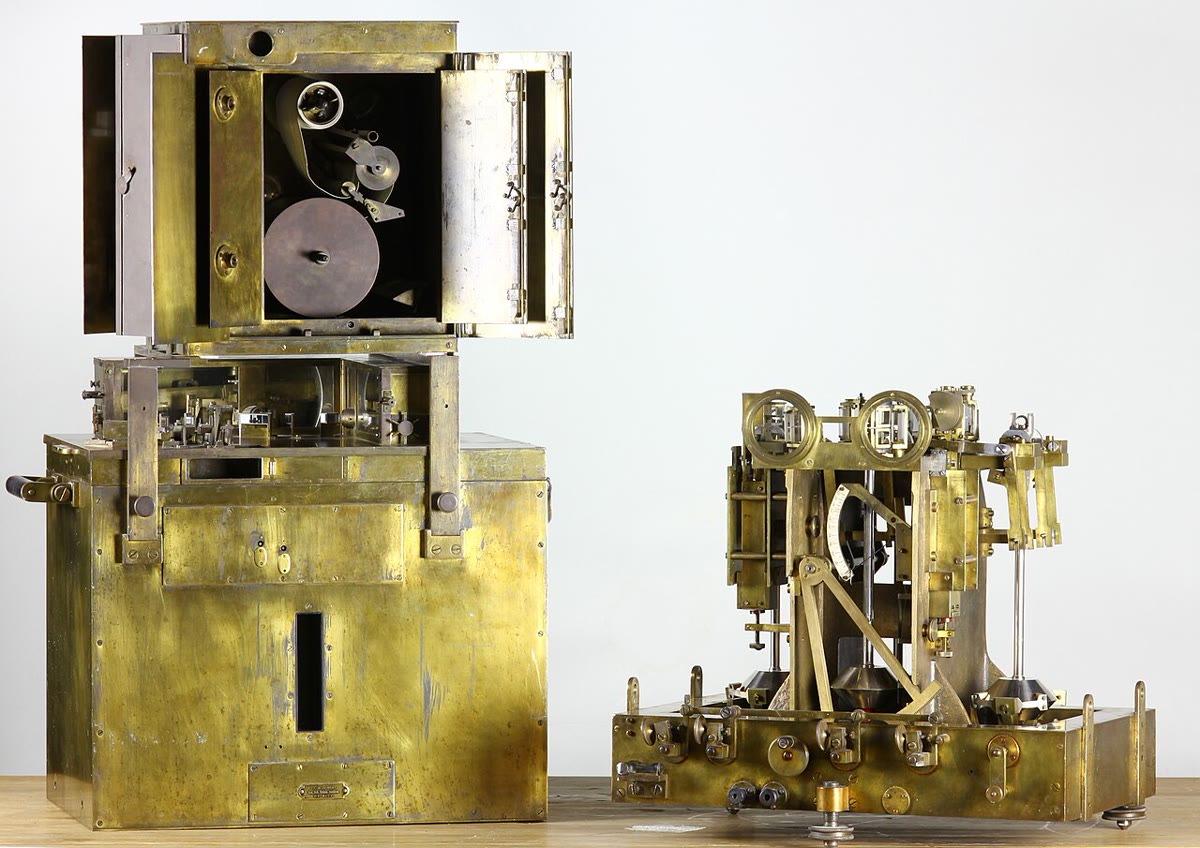
\includegraphics[width=\linewidth]{images/book3/b1-vening-meinesz.jpg}

{\scriptsize جهاز بندول فينينغ مينيز (يمين) وعلبته مع وحدة التسجيل (Broodt, CC BY-SA 4.0).}
\end{minipage}
\end{history}

\section{الجيود}

سطح البحر الساكن سطح ذو جهد ثقالي ثابت: فلو لم يكن كذلك لجرى الماء على امتداده. وهو المرجع الطبيعي للارتفاعات، وهو السطح الذي كانت الشواقيل القديمة عمودية عليه.

\begin{definition}[الجيود؛ ارتفاع الجيود]\label{def:b1:isostasy-gravity:geoid}
\emph{الجيود}\index{الجيود} هو سطح تساوي الجهد لجاذبية الأرض (الجذب الثقالي مع الأثر الطارد المركزي للدوران)، الذي يُطابق متوسط سطح البحر فوق المحيطات المفتوحة في حال السكون، ويُمدّ تحت القارات. و\emph{ارتفاع الجيود}\index{ارتفاع الجيود} $N$ عند نقطة هو ارتفاع الجيود فوق القطع الناقص المرجعي، ويُعدّ سالبًا حيث يقع الجيود تحته.
\end{definition}

الارتفاعات فوق مستوى البحر على الخرائط هي ارتفاعات فوق \omterm{def:b1:isostasy-gravity:geoid}{الجيود}؛ أما الارتفاعات التي يعطيها تحديد المواقع بالأقمار الصناعية فهي ارتفاعات فوق القطع الناقص؛ والفرق بينهما $N$. ويبتعد \omterm{def:b1:isostasy-gravity:geoid}{الجيود} عن القطع الناقص بمقدار \qty{+85}{m} قرب أيسلندا، و\qty{-106}{m} قبالة جنوب الهند، وأقل من \qty{200}{m} في المجموع، بينما يمتدّ تضاريس السطح الصلب نحو \qty{20}{km}: \omterm{def:b1:isostasy-gravity:geoid}{فالجيود} سطح أملس بكثير من سطح الأرض.
% ledger: nasa:geoid-range, earth:topo

\begin{proposition}[ارتفاع الجيود وشذوذ الجهد]\label{prop:b1:isostasy-gravity:bruns}
ليكن $\Phi$ جهد جاذبية الأرض، و$\Phi_n$ الجهد المرجعي، أي جهد الأرض النموذجية التي يكون سطحها، القطع الناقص المرجعي، ذا الجهد $\Phi_0$ نفسه الذي للجيود، معدودَين بإشارة الفيزياء (يزداد الجهد نحو الأعلى، و$g = -\nabla\Phi$). وليكن $T = \Phi - \Phi_n$ شذوذ الجهد عند \omterm{def:b1:isostasy-gravity:geoid}{الجيود}. وبالتقريب من الرتبة الأولى،
\[
  N = -\frac{T}{\gamma} .
\]
أما الجيوديسيون، الذين يعدّون الجهد بإشارة معاكسة، فيكتبون النتيجة نفسها $N = T/\gamma$، وهي صيغة برونز.
\end{proposition}

\begin{proof}
ليكن $Q$ نقطة من القطع الناقص، و$P$ نقطة \omterm{def:b1:isostasy-gravity:geoid}{الجيود} على الناظم المار بالنقطة $Q$، على الارتفاع $N$. يزداد الجهد المرجعي نحو الأعلى بمعدّل $\gamma$، إذن $\Phi_n(P) \approx \Phi_n(Q) + \gamma N = \Phi_0 +
\gamma N$. ولما كانت $P$ على \omterm{def:b1:isostasy-gravity:geoid}{الجيود}، فإن $\Phi(P) = \Phi_0$، أي $\Phi_n(P) + T = \Phi_0$. ومنه $\Phi_0 + \gamma N + T = \Phi_0$ و$N =
-T/\gamma$.
\end{proof}

يجعل فائض الكتلة تحت نقطة ما الجهدَ هناك أكثر سلبيةً، إذن $T < 0$ و$N > 0$: ينتفخ \omterm{def:b1:isostasy-gravity:geoid}{الجيود} فوق فائض الكتلة ويغوص فوق العجز. ويقابل الارتفاع \qty{85}{m} قرب أيسلندا شذوذ جهد قدره $-\qty{85}{m}\times\qty{9.8}{m.s^{-2}} \approx \qty{-830}{J.kg^{-1}}$. ولأن الجهد يتناقص كما $1/r$، بينما تتناقص الجاذبية كما $1/r^2$، فإن \omterm{def:b1:isostasy-gravity:geoid}{الجيود} تهيمن عليه الكتل الكبيرة العميقة، والشذوذات الثقالية تهيمن عليها الكتل الضحلة. ولا ترفع سلسلة جبلية معوَّضة \omterm{def:b1:isostasy-gravity:geoid}{الجيود} إلا قليلًا، لأن فائض كتلتها وعجز جذرها يتلاشيان تقريبًا؛ أما الحمل غير المعوَّض فيرفعه أكثر بكثير.

\begin{omfigure}
\begin{tikzpicture}[x=1.15cm, y=1.3cm, font=\scriptsize, >={Stealth[length=4pt]}]
% schematic, not to scale
\fill[omSea!35] (0,0.05) .. controls (1.5,0.25) and (2.5,0.35) .. (3.6,0.45) -- (3.6,-1.2) -- (0,-1.2) -- cycle;
\fill[omLithGranite!40] (3.6,0.45) .. controls (4.5,1.4) and (5.4,1.9) .. (6.4,1.7) .. controls (7.4,1.5) and (8.2,1.2) .. (9,1.0) -- (9,-1.2) -- (3.6,-1.2) -- cycle;
\fill[omLithGabbro!35] (0,-0.7) .. controls (1.2,-0.9) and (2.4,-0.6) .. (3.6,-0.2) -- (3.6,-1.2) -- (0,-1.2) -- cycle;
\draw[thick, blue!70!black] (0,0.05) .. controls (1.5,0.25) and (2.5,0.35) .. (3.6,0.45) .. controls (5,0.75) and (7,0.75) .. (9,0.55);
\draw[thick, black, densely dashed] (0,-0.25) .. controls (3,0.05) and (6,0.15) .. (9,0.1);
\draw (3.6,0.45) .. controls (4.5,1.4) and (5.4,1.9) .. (6.4,1.7) .. controls (7.4,1.5) and (8.2,1.2) .. (9,1.0);
\node[anchor=west, blue!70!black] at (9.05,0.6) {الجيود};
\node[anchor=west] at (9.05,0.1) {القطع الناقص};
\node[anchor=west] at (9.05,1.0) {سطح الأرض};
\node at (1.4,-0.3) {المحيط};
\node at (1.6,-1.0) {قاع البحر};
% heights (curve ordinates computed from the Bezier segments)
\draw[<->] (6.6,0.107) -- (6.6,0.688); \node[anchor=east] at (6.57,0.40) {$N$};
\draw[<->] (7.2,0.674) -- (7.2,1.512); \node[anchor=west] at (7.23,1.09) {$H$};
\draw[<->] (8.2,0.110) -- (8.2,1.224); \node[anchor=east] at (8.17,0.95) {$h_e$};
% the vertical (perpendicular to the geoid) and the ellipsoid normal at x = 2.4 (angle exaggerated)
\draw[->, thick, blue!70!black] (2.4,0.335) -- (2.0,1.3);
\draw[->, thick, black] (2.4,0.335) -- (2.33,1.3);
  \node[anchor=south east, blue!70!black] at (2.05,1.3) {الشاقول};
  \node[anchor=south west] at (2.3,1.3) {ناظم القطع الناقص};
\end{tikzpicture}

\par\smallskip{\small \omterm{def:b1:isostasy-gravity:geoid}{الجيود} (باللون الأزرق)، والقطع الناقص المرجعي (المتقطّع)، والأرض (تخطيطيًا؛ والانحرافات مبالغ فيها بشدة). فوق المحيط يكون \omterm{def:b1:isostasy-gravity:geoid}{الجيود} سطح البحر الساكن؛ وتحت اليابسة يُمدّ سطحًا لتساوي الجهد. يُقاس الارتفاع $H$ على الخريطة من \omterm{def:b1:isostasy-gravity:geoid}{الجيود}، ويُقاس الارتفاع $h_e$ الذي يعطيه تحديد المواقع بالأقمار الصناعية من القطع الناقص، و$h_e = H + N$. والشاقول عمودي على \omterm{def:b1:isostasy-gravity:geoid}{الجيود} لا على القطع الناقص: والزاوية بينهما (مبالغ فيها هنا) هي انحراف الشاقول الذي أقلق المساحين في الهند.}
\label{fig:b1:isostasy-gravity:geoid}
\end{omfigure}

الانحرافات صغيرة: فالتناقض كله الذي أقلق مساحي الهند كان نحو خمس ثوانٍ قوسية. وفوق المحيطات يُرى \omterm{def:b1:isostasy-gravity:geoid}{الجيود}.
ومنذ 1978 تقيس مقاييس الارتفاع الرادارية على الأقمار الصناعية زمن نبضات الموجات الدقيقة المنعكسة عن سطح البحر لتقيس ارتفاعه. وبعد تصفية المدّ والأمواج والتيارات بالمتوسط، يعلو سطح البحر فوق الجبال البحرية والحيود، ويهبط فوق الأخاديد والسهول القاعية، وهذه الانتفاخات (\cref{exo:b1:isostasy-gravity:11} يقدّر إحداها) ترسم تضاريس قاع المحيط العميق حيث لم تسبره سفينة قط. والقمر الصناعي GOCE، من 2009 إلى 2013، طار على ارتفاع نحو \qty{260}{km} وقاس حقل الجاذبية من المدار، قاصدًا \omterm{def:b1:isostasy-gravity:geoid}{الجيود} بدقة من 1 إلى \qty{2}{cm}، والشذوذات الثقالية بدقة نحو \qty{1}{\milli\gal}، مع تحليل أفضل من \qty{100}{km}.
% ledger: pratt:himalaya, jpl:seasat, esa:goce

\subsection*{التوازن الأيزوستاتي في الحركة}

يُبلَغ \omterm{def:b1:isostasy-gravity:isostasy}{التوازن الأيزوستاتي} بالتدفّق، والتدفّق يستغرق زمنًا. وفي ذروة آخر عصر جليدي، قبل نحو \num{20000} سنة، غطّت صفيحة جليدية سمكها نحو \qty{3}{km} اسكندنافيا.
كثافة الجليد نحو تسعة أعشار كثافة الماء، فمع \omterm{def:b1:layered-earth:layers}{وشاح} كثافته \qty{3300}{kg.m^{-3}} يكون الهبوط الأيزوستاتي الكامل تحت صفيحة كهذه $\qty{3000}{m}\times900/3300 \approx \qty{820}{m}$. وقد زال الجليد، والأرض ما زالت ترتفع: يقيس تحديد المواقع بالأقمار الصناعية ارتفاعًا يبلغ نحو \qty{10}{mm.yr^{-1}} في شمال السويد، غرب خليج بوثنيا، اليوم. ومعدّل استرخاء الهبوط يقيس لزوجة \omterm{def:b1:layered-earth:layers}{الوشاح} تحته، وهي موضوع الكتاب 5؛ ويبيّن \cref{exo:b1:isostasy-gravity:12} الطريقة.
% ledger: kierulf:fennoscandia, usgs:ice-density

\section{التمارين}

\begin{exercise}[$\star$]\label{exo:b1:isostasy-gravity:1}
(أ) حوّل \omterm{def:b1:isostasy-gravity:anomalies}{شذوذ بوغيه} البالغ \qty{-150}{\milli\gal} إلى \unit{m.s^{-2}}، وعبّر عنه كنسبة من $g = \qty{9.81}{m.s^{-2}}$. (ب) افعل الأمر نفسه مع \qty{1}{\milli\gal}، وهي الدقة المستهدفة لشذوذات الجاذبية من GOCE، ومع \qty{1}{\micro\gal}.
% ledger: esa:goce, nist:gal
\end{exercise}

\begin{exercise}[$\star$]\label{exo:b1:isostasy-gravity:2}
(أ) احسب \omterm{def:b1:isostasy-gravity:normal-gravity}{الجاذبية المرجعية} عند خط الاستواء، وعند \ang{45}، وعند القطبين بصيغة الفصل. (ب) أعطِ الفرق من خط الاستواء إلى القطب بالميليغال. (ج) التسارع الطارد المركزي عند خط الاستواء هو \qty{3392}{\milli\gal}. ما كسر الفرق الذي يفسّره الدوران مباشرة؟
% ledger: moritz:grs80
\end{exercise}

\begin{exercise}[$\star$]\label{exo:b1:isostasy-gravity:3}
ترتفع هضبة \qty{3}{km} فوق مستوى البحر. ومع \omterm{def:b1:layered-earth:layers}{قشرة} كثافتها \qty{2800}{kg.m^{-3}} \omterm{def:b1:layered-earth:layers}{ووشاح} كثافته \qty{3300}{kg.m^{-3}}، احسب جذر إيري الخاص بها، والزيادة في سمك قشرتها.
\end{exercise}

\begin{exercise}[$\star$]\label{exo:b1:isostasy-gravity:4}
(أ) بكم يجب أن يُرفع مقياس الجاذبية لينخفض قراؤه بمقدار \qty{1}{\milli\gal}؟ استعمل \qty{0.3086}{\milli\gal.m^{-1}}. (ب) يهدف مسح إلى شذوذات دقتها \qty{0.01}{\milli\gal}. إلى أي دقة يجب أن تُعرف ارتفاعات المحطات؟
\end{exercise}

\begin{exercise}[$\star\star$]\label{exo:b1:isostasy-gravity:5}
في نموذج برات، مع $D = \qty{100}{km}$ و$\rho_0 = \qty{2700}{kg.m^{-3}}$، (أ) احسب كثافة الأعمدة التي ترتفع \qty{1}{km} و\qty{3}{km} و\qty{5}{km}؛ (ب) احسب كثافة عمود تحت \qty{4}{km} من ماء البحر كثافته \qty{1030}{kg.m^{-3}}. (ج) لماذا يلائم نموذج برات قاع المحيط أكثر مما يلائم القارات؟
\end{exercise}

\begin{exercise}[$\star\star$]\label{exo:b1:isostasy-gravity:6}
تقع محطتان عند \omterm{def:b1:spherical-astronomy:geographic}{العرض الجغرافي} \ang{48}، حيث \omterm{def:b1:isostasy-gravity:normal-gravity}{الجاذبية المرجعية} \qty{9.808911}{m.s^{-2}}. المحطة 1، على ارتفاع \qty{350}{m} فوق مستوى البحر، تعطي \qty{9.807751}{m.s^{-2}}، والمحطة 2، على \qty{1850}{m}، تعطي \qty{9.803552}{m.s^{-2}}. (أ) احسب شذوذي الهواء الحر وبوغيه لكلتيهما، بكثافة بوغيه المعيارية. (ب) ماذا تقترح شذوذات المحطة 2 عن الجبال المحيطة بها؟
\end{exercise}

\begin{exercise}[$\star\star$]\label{exo:b1:isostasy-gravity:7}
(أ) على غرار برهان \cref{prop:b1:isostasy-gravity:slab}، أثبت أن قرصًا أفقيًا نصف قطره $a$ وسمكه $h$ وكثافته $\rho$ يجذب نقطة على محوره، على بعد $z \gg h$ فوقه، بمقدار $2\pi G\rho h\,\bigl(1 -
z/\sqrt{z^2 + a^2}\bigr)$. (ب) أي نصف قطر يعطي \qty{90}{\percent} من قيمة الصفيحة عند $z = \qty{1}{km}$؟ (ج) ماذا يعني ذلك لمساحة التضاريس التي تهمّ \omterm{def:b1:isostasy-gravity:anomalies}{تصحيح بوغيه}؟
\end{exercise}

\begin{exercise}[$\star\star$]\label{exo:b1:isostasy-gravity:8}
في نموذج إيري، مع \omterm{def:b1:layered-earth:layers}{قشرة} كثافتها \qty{2800}{kg.m^{-3}} وسمكها \qty{35}{km} عند مستوى البحر، فوق \omterm{def:b1:layered-earth:layers}{وشاح} كثافته \qty{3300}{kg.m^{-3}}، (أ) احسب الجذر المعكوس وسماكة \omterm{def:b1:layered-earth:layers}{القشرة} تحت \qty{4}{km} من ماء البحر كثافته \qty{1030}{kg.m^{-3}}. (ب) \omterm{def:b1:layered-earth:layers}{القشرة} المحيطية سمكها نحو \qty{5}{km} في الواقع. ماذا يبيّن الفرق؟ % ledger: usgs:crust-thickness
\end{exercise}

\begin{exercise}[$\star\star$]\label{exo:b1:isostasy-gravity:9}
في وصف المقدمة، كان التناقض في الفرق في \omterm{def:b1:spherical-astronomy:geographic}{العرض الجغرافي} بين كاليانا وكاليانبور \qty{5.236}{''}، بينما كان جذب الهملايا الذي حسبه برات يجب أن ينتج \qty{15.885}{''}. (أ) حوّل الزاويتين إلى راديان. (ب) يميل تسارع أفقي $a_h$ الشاقول بالزاوية $a_h/g$. ما فرق الجذب الأفقي بين المحطتين الذي تقابله كل زاوية، بالميليغال، مع $g = \qty{9.79}{m.s^{-2}}$؟ (ج) ما كسر جذب الجبال المرئية الذي ألغاه التعويض؟
% ledger: pratt:himalaya
\end{exercise}

\begin{exercise}[$\star\star\star$]\label{exo:b1:isostasy-gravity:10}
يُمثَّل قبّة ملحية بكرة نصف قطرها \qty{2}{km}، ومركزها على عمق \qty{4}{km}، بكثافة أقل بمقدار \qty{200}{kg.m^{-3}} من الصخور المحيطة بها. (أ) أثبت أن كرة مدفونة ذات كتلة شاذة $M$ على عمق $z$ تعطي، على المسافة الأفقية $x$، الشذوذ $GMz/(x^2 + z^2)^{3/2}$. (ب) احسب الشذوذ فوق مركزها. (ج) على أي مسافة ينخفض إلى نصف قيمته القصوى؟ (د) كيف يمكن قراءة عمق الكرة من قطاع مقاس؟
\end{exercise}

\begin{exercise}[$\star\star\star$]\label{exo:b1:isostasy-gravity:11}
سفح بحري هو مخروط ارتفاعه \qty{3}{km} وقاعدته نصف قطرها \qty{15}{km}، قائم على قاع بحر عمقه \qty{5}{km}. وكثافة صخره \qty{2800}{kg.m^{-3}}، وكثافة ماء البحر \qty{1030}{kg.m^{-3}}. (أ) احسب كتلته الزائدة على الماء الذي يزيحه. (ب) عامله كنقطة كتلة في مركز كتلته، على ربع ارتفاعه فوق القاعدة، واستعمل \cref{prop:b1:isostasy-gravity:bruns} مع $\gamma = \qty{9.81}{m.s^{-2}}$ لتقدير ارتفاع الانتفاخ الذي يحدثه في سطح البحر فوقه. (ج) هل تبالغ نقطة الكتلة في تقدير الانتفاخ أم تقلّل منه؟ (د) لو كان السفح معوَّضًا بجذر تعويضًا كاملًا، كيف يتغيّر الانتفاخ؟
\end{exercise}

\begin{exercise}[$\star\star\star$]\label{exo:b1:isostasy-gravity:12}
نمذج استعادة اسكندنافيا بعد زوال الجليد: لنفترض أن الجليد زال فجأة قبل \num{10000} سنة، تاركًا هبوطًا قدره \qty{818}{m} نقص منذ ذلك الحين وفق $w(t) = w_0\,e^{-t/\tau}$. (أ) أثبت أن معدّل الرفع هو $w/\tau$. (ب) مع $\tau = \num{4000}$ سنة، احسب الهبوط المتبقي ومعدّل الرفع اليوم، وقارن المعدّل بالقيمة المقاسة \qty{10}{mm.yr^{-1}}. (ج) أثبت أن $\tau = \num{3100}$ سنة و$\tau = \num{68000}$ سنة يعطيان كلاهما نحو \qty{10}{mm.yr^{-1}} اليوم. ما الهبوط المتبقي الذي يقتضيه كل منهما، وكيف يمكن لمسح للجاذبية أن يفصل بينهما؟ (د) ما الخاصية في \omterm{def:b1:layered-earth:layers}{الوشاح} التي يقيسها $\tau$؟
% ledger: kierulf:fennoscandia
\end{exercise}

\section{مسألة: جذر سلسلة جبلية}

\begin{problem}[{مسألة نهاية الأسبوع: جذر الهضبة، وإيري في مواجهة برات، والجاذبية فوقها، وما تفعله التعرية بها}]
\label{pb:b1:isostasy-gravity:1}
% values: calc/ch11.py (invented plateau; normal gravity formula of the chapter)
% ledger: moritz:grs80, usgs73:reduction
هضبة واسعة، عرضها عدة مئات من الكيلومترات، ترتفع \qty{4}{km} فوق منخفض عند مستوى البحر سمك قشرته \qty{35}{km}. خذ $\rho_c = \qty{2700}{kg.m^{-3}}$ \omterm{def:b1:layered-earth:layers}{للقشرة}، و$\rho_m = \qty{3300}{kg.m^{-3}}$ \omterm{def:b1:layered-earth:layers}{للوشاح}، و$g = \qty{9.81}{m.s^{-2}}$، و$2\pi G = \qty{0.0419}{\milli\gal}$ لكل متر ولكل \qty{1000}{kg.m^{-3}}.

\medskip
\noindent\textbf{الجزء الأول --- هضبة إيري.}
\begin{enumerate}
  \item احسب جذر إيري للهضبة.
  \item استنتج سمك قشرتها، وعمق \omterm{def:b1:layered-earth:discontinuity}{موهو} تحت مستوى البحر.
  \item خذ \omterm{def:b1:isostasy-gravity:isostasy}{عمق التعويض} على \qty{60}{km} تحت مستوى البحر. احسب الكتلة لكل متر مربع فوقه في عمود الهضبة وفي عمود المنخفض.
  \item احسب الضغط على عمق \qty{60}{km}.
  \item لماذا يساوي الجذر \num{4.5} مرات الارتفاع؟ ما النسبة لو كانت كثافة \omterm{def:b1:layered-earth:layers}{القشرة} \qty{2900}{kg.m^{-3}}؟
  \item ماذا يُظهر مسح انكسار زلزالي عبر حافة الهضبة لو صحّ نموذج إيري؟
\end{enumerate}

\noindent\textbf{الجزء الثاني --- هضبة برات.}
لنفترض بدلًا من ذلك عمق تعويض $D = \qty{100}{km}$ تحت مستوى البحر، وعمودًا للمنخفض كثافته منتظمة \qty{2700}{kg.m^{-3}}.
\begin{enumerate}[resume]
  \item احسب كثافة عمود الهضبة.
  \item تحقّق من أن للعمودين الكتلة نفسها لكل متر مربع فوق $D$.
  \item بكم بالمئة يجب أن يكون عمود الهضبة أخفّ؟
  \item لو كان فرق الكثافة هذا ناجمًا عن الحرارة وحدها، بمعامل تمدّد حراري قدره \qty{3e-5}{K^{-1}}، فكم يجب أن يكون عمود الهضبة أسخن في المتوسط؟ هل هذا معقول؟
  \item أين يقع \omterm{def:b1:layered-earth:discontinuity}{موهو} تحت الهضبة في نموذج برات؟
  \item يجد مسح انكساري أن \omterm{def:b1:layered-earth:discontinuity}{موهو} يقع على \qty{52}{km} تحت الهضبة. أيّ النموذجين يطابق ذلك؟
\end{enumerate}

\noindent\textbf{الجزء الثالث --- الجاذبية فوق المركز.}
\begin{enumerate}[resume]
  \item احسب \omterm{def:b1:isostasy-gravity:anomalies}{تصحيح بوغيه} لمحطة على الهضبة.
  \item توقّع شذوذي الهواء الحر وبوغيه عند المركز لو لم تكن الهضبة معوَّضة.
  \item توقّعهما لهضبة إيري، وتحقّق من \omterm{def:b1:isostasy-gravity:anomalies}{شذوذ بوغيه} بكتلة الجذر الناقصة.
  \item محطة عند مركز الهضبة، عرضها الجغرافي \ang{30} وارتفاعها \qty{4000}{m}، تعطي \qty{9.781085}{m.s^{-2}}. احسب \omterm{def:b1:isostasy-gravity:normal-gravity}{الجاذبية المرجعية} عند \ang{30}، ثم شذوذي الهواء الحر وبوغيه.
  \item ما كسر الهضبة المعوَّض؟
  \item هل يختلف \omterm{def:b1:isostasy-gravity:anomalies}{شذوذ بوغيه} عند المركز لو عُوِّضت الهضبة بطريقة برات؟ علّل.
  \item ارسم تخطيطيًا \omterm{def:b1:isostasy-gravity:anomalies}{شذوذ الهواء الحر} على قطاع عبر إحدى حواف الهضبة، وفسّر شكله.
\end{enumerate}

\noindent\textbf{الجزء الرابع --- التعرية.}
تُزيل الأنهار طبقة سمكها \qty{1}{km} من سطح الهضبة كله، ببطء يكفي لأن يواكبها \omterm{def:b1:isostasy-gravity:isostasy}{التوازن الأيزوستاتي}.
\begin{enumerate}[resume]
  \item ما السمك الجديد \omterm{def:b1:layered-earth:layers}{للقشرة}، وما جذر إيري الجديد لها؟
  \item ما الارتفاع الجديد للهضبة؟
  \item بكم ارتفعت الصخور التي صارت الآن على السطح؟
  \item كم من الصخر يجب أن تُزيله التعرية في المجموع لتنزل الهضبة إلى مستوى البحر؟ ماذا يقول هذا عن الصخور التي تُرى في أحزمة الجبال القديمة؟
  \item بكم ينخفض سطح الهضبة مقابل كل كيلومتر من الصخر المُزال؟
\end{enumerate}
\end{problem}
